\begin{resume}
La gestion de l'hétérogénéité des ressources peut être considérée sous plusieurs aspects. Les chapitres précédents ont donné des exemples de travaux dans lesquels l'hétérogénéité s'était concentrée sur les communications (Chapitre \ref{Chap:MPI}) ou sur le couple données-communication (Chapitre \ref{SEC:GRAPPES}). Dans ce chapitre nous nous concentrons sur un troisième socle, celui de l'hétérogénéité de calcul. Plus exactement, ce chapitre présente des travaux dont les contributions ont visé la prise en charge de l'hétérogénéité des ressources de calcul ou l'hétérogénéité des tâches de calcul, tous les deux résultant en une variabilité des temps d'éxécution de tâches qui a dû être traitée et optimisée. Il est aussi important de remarquer que la communication et le stockage peuvent varier mais, dans ces cas, ils sont traités par des outils et mécanismes sous-jacents qui n'ont pas été la cîble de nos travaux.

Ainsi, ce chapitre démarre avec la description d'une plate-forme de calcul destinée à l'exécution de problèmes d'amarrage moléculaire. Ce travail, développé dans le cadre de la co-direction de thèse de Romain Vasseur, est un exemple d'application métier où l'environnement développée sert à déployer de manière distribuée une application déjà existante et dont le code source ne pourrait pas être facilement parallélisée. L'approche retenue a été composée d'une gestion distribuée d'instances de calcul sur un cluster/grappe, associée à un découpage plus fin du problème afin de multiplier les tâches de calcul et ainsi mieux utiliser les ressources disponibles.

La deuxième partie de ce chapitre décrit les efforts effectués dans le cadre du projet de collaboration international STIC-AmSud PER-MARE, dont l'un des objectifs a été de rendre la plateforme de calcul big data Hadoop sensible au contexte et donc capable d'adapter la distribution des tâches de calcul en fonction des variations des ressources.

\end{resume}

\section{Hétérogénéité des Tâches  - application à la recherche en amarrage moléculaire} \label{sec:Vasseur}

L'usage d'approches informatiques pour identifier les interactions biomoleculaires est devenu l'un des principaux piliers de la recherche de nouvelles drogues et principes actifs. En effet, la simulation \emph{in silico} permet de faire une première prospection sur un grand nombre de candidats potentiels, tout avec un gain de temps important et un coût nettement moins onéreux que l'expérimentation \emph{in vitro}. 

L'amarrage moléculaire (aussi appelé \emph{docking moléculaire)}) est donc une technique qui vise à étudier les interactions au niveau moléculaire entre certaines structures du vivant, comme par exemple les interactions protéine-ADN/ARN, protéine-protéine, peptides-protéine, protéine-ligand ou glucide-protéine. L'industrie pharmaceutique s'intéresse particulièrement par l'étude des interactions protéine-ligand, notamment à la recherche de petites molécules chimiques comme les principes actifs de médicaments (ligands) qui puissent se connecter à certaines protéines cible. La prédiction des modes d'amarrage d'un ligand à une protéine, la structure du complexe résultant et l'estimation de l'affinité de cet amarrage sont essentiels pour le développement de nouveaux composés thérapeutiques, et les méthodes numériques ont été le choix principal de plusieurs travaux dans la littérature \cite{1}\cite{9}\cite{19}.

 Souvent cette étude se fait à travers un "criblage virtuel" (\emph{virtual screening}), qui consiste au déploiement à grande échelle permettant de tester un grand nombre de ligands (de centaines à plusieurs millions selon l’ampleur de la campagne) sur un nombre très restreint de cibles. En effet, nous trouvons des millions de composants catalogués dans des bases de données de chimie telles que la Cambridge Structural Database \cite{2}, PDBbind  \cite{27} \cite{28}, ZINC \cite{16} et tant d'autres collections privées des groupes pharmaceutiques. De même, un extense catalogue de protéines peut être obtenu à partir du Research Collaboratory for Structural Biology (RCSB) Protein Data Bank (PDB) \cite{26}, une base de données ouverte qui contient plus de 120 mille protéines cataloguées et qui est enrichie de plus de 7000 nouvelles protéines par an. Ainsi, un chercheur ou un industriel qui souhaite activer ou désactiver une protéine afin de combattre une maladie peut donc effectuer ce criblage virtuel entre la protéine cible et les milliers de ligands catalogués (enzymes, peptides, etc.).  

Dans le cadre des travaux de thèse de Romain Vasseur (thèse en bio-informatique, dirigée par le prof. Manuel Dauchez et co-encadré par Stéphanie Baud et moi-même) nous nous sommes penchés sur le développement et exécution parallèle d'une application pour le criblage moléculaire inversé. Plus exactement, un criblage inversé a pour objectif de discriminer les cibles protéiques les plus favorables à une interaction avec le ligand, parmi un échantillon de structures de protéines plus ou moins important. De cette manière, il est possible d'identifier des cibles secondaires pour un ligand développé, ou bien faire une étude préalable des risques d'interactions indésirables. 

\subsection{Travaux proches et métodologie de parallélisation}
%TODO ref
Le terme “inverse docking” a fait son apparition dans la littérature en 2001 avec les deux articles de Chen et al. [164][165]. Une quinzaine d'articles ont été recensés depuis cette date, avec des méthodes de traitement à plus ou moins grande échelle. La plupart de ces travaux font l'usage d'applications pour le docking traditionnel telles que AutoDock [172] ou AutoDock Vina [173] [174], et très peu d'outils sont dédiés au docking inversé (INVDOCK [164] [165] ou TarFisDock [177]). Toutefois, aucun de ces articles ne mentionne ni le déploiement ni le développement d’une méthode de déploiement sur des architectures de type HPC.

Ainsi, nous avons développé nos propres stratégies dans le but de pouvoir traiter des centaines en parallèle de protéines grâce aux architectures HPC.
Ces stratégies concernent la parallélisation du calcul d'un couple ligand-protéine mais aussi le déploiement large échelle de ces calculs. 

Dans ce travail nous sommes parti de la méthode appelée "Blind docking" qui consiste à détecter des points d'amarrage possibles en faisant un balayage sur l'ensemble de la surface de la protéine. Pour cela, des applications telles que Autodock doivent générer une grille d'affinités basée sur les énergies de liaison de chaque atome qui compose la protéine. Cette grille d'affinité représente une boîte 3D qui contient toute la surface de la protéine (plus une marge afin de permettre le placement d'un ligand à l'intérieur de la boîte),  et un algorithme génétique ira explorer le volume autour de la protéine afin d'évaluer l'énergie de liaison de différents points. Bien sûr, cette approche naïve est difficilement parallélisable car chaque pair protéine-ligand représente une boîte et donc une tâche de calcul Autodock. De plus, selon les caractéristiques de la protéine, un nombre important de tours (générations dans l'algorithme génétique) sont nécessaires pour couvrir systématiquement la surface de la protéine et permettre l'obtention de résultats satisfaisants. Comme résultat, l'exécution d'une seule instance de "blind docking" avec l'application AutoDock peut prendre plusieurs heures.

%TODO imagem com um box de blind dockinh

Malgré ces contraintes, cette approche est assez répandue et a donc été utilisée comme référence de comparaison pour les approches parallèles que nous avons développé.

\subsection{Parallélisme Intérieur : décomposition des tâches}
Afin d'optimiser l'utilisation des ressources de calcul lors d'une campagne de docking inversé, il est impératif d'intégrer le parallélisme au cœur du traitement des tâches de calcul, comme illustré en figure \ref{fig:romain-fig1}. La décomposition d'une instance de docking permet de mieux utiliser les ressources de calcul en distribuant les tâches sur plusieurs machines, mais aussi grâce à un traitement en pipeline qui permet l'enchaînement des opérations lorsque certaines tâches finissent plus tôt. De plus, cela rend l'exécution plus tolérante aux fautes, une tâche qui a été interrompue peut être redéployée sur une autre machine sans obliger le redémarrage de toute l'exécution. Dans le cadre de ce travail, nous avons étudié les techniques de décomposition présentées dans les sections suivantes. 

\begin{figure}
	\begin{center}
		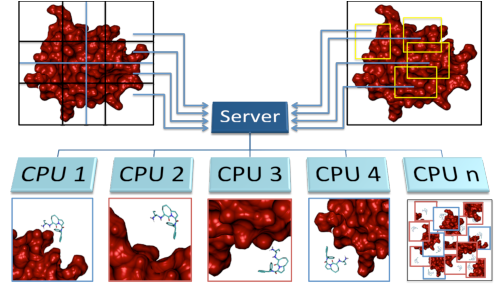
\includegraphics[width=0.85\linewidth]{images/Romain/fig1-color}
	\end{center}
	\caption{Exemple d'un schéma de décomposition parallèle}\label{fig:romain-fig1}
\end{figure}

\subsubsection{Décomposition géométrique arbitraire}
Vu la nature des données utilisées en entrée pour le docking, nous avons initialement étudié une stratégie de décomposition géométrique qui consiste à découper la grille d'affinité 3D en plusieurs boîtes plus petites, chacune couvrant un secteur de la protéine. Cette stratégie considère une décomposition géographique régulière de telle manière que le nombre de tâches (boîtes) ont une taille similaire, permettant ainsi la génération de $n^3$ sous-grilles : 8 (2x2x2), 27 (3x3x3), 64 (4x4x4), etc. Le choix du bon nombre de découpages dépend à la fois du gain  en parallélisme mais aussi de la liberté de mouvement du ligand à l'intérieur d'une grille. 
En effet, on peut espérer un gain de performance dans le fait de pouvoir déployer en parallèle les différentes sous-grilles comme des tâches de calcul indépendantes, toutefois un nombre trop important de découpages aura par effet la génération de sous-grilles "inutiles" car elles couvrent que des zones inaptes à la recherche de points d'amarrage (espace non connecté à la surface de la protéine, "intérieur" de la protéine, etc.). De plus, une boîte 3D trop petite peut empêcher le positionnement du ligand et donc rendre l'évaluation de l'amarrage impossible.

Un autre inconvénient de cette technique est que le découpage se fait de manière arbitraire, sans prendre en compte les spécificités de la surface de la protéine. Par exemple, les "cavités" présentes dans la surface de la protéine sont souvent des bons sites pour l'amarrage, mais un découpage arbitraire qui l'ignore peut simplement scinder cette cavité en deux et la rendre bien moins intéressante vis-à-vis de l'algorithme de docking. De même, l'évaluation de docking se fait à en considérant que le ligant se trouve totalement à l'intérieur de la sous-grille : n'importe quelle conformation où des atomes ligand dépassent la grille serait invalidée et donc ignorée. 

\subsubsection{Décomposition Géométrique avec superposition}
Les inconvénients de la décomposition géométrique arbitraire cités dans le section précédente nous ont conduit à développer une technique alternative de découpage qui préserve la liberté de placement des ligands et permet une couverture intégrale de la surface de la protéine. Cette technique consiste à effectuer un découpage avec superposition entre les sous-grilles voisines, de manière à pouvoir évaluer le placement du ligand même sur les zones proches des bords des sous-grilles. Bien sûr, cette superposition est dépendante de la taille des ligands, permettant ainsi une configuration qui optimise l'utilisation des ressources pour chaque pair protéine-ligand. 

Ainsi, dans le cadre du travail effectué, nous avons considéré deux valeurs de référence pour la superposition. La superposition entre deux boîtes serait d'un tiers de la longueur de la boîte si la longueur du ligand est inférieure à cela. Dans le cas contraire, la superposition correspond à la longueur du ligand. Grâce à cette configuration, le ligand a une liberté complète de placement (rotation, translation, etc.) et on peut effectuer une recherche exhaustive sur l'espace d'amarrage. Dans l'exemple illustré dans les prochaines sections nous utilisons aussi un schéma de décomposition en douze parties, 3x2x2 (où 3 correspond à l'axe principal de la protéine) et avec une superposition d'1/3 sur chaque sous-grille. 

\subsubsection{Recherche de cavités}
Comme indiqué précédemment, l'amarrage des ligands est favorisée par la présence de cavités dans la surface de la protéine [34][35], or les méthodes de découpage par décomposition ne prennent pas ces facteurs en compte. En effet, même avec la décomposition avec superposition, l'algorithme génétique utilisé pour la recherche de points d'amarrage ne fait que parcourir la surface sans un objectif définit. 

La détection des zones avec cavités se fait à partir d'un programme extérieur, Fpocket [36], spécialisé dans la recherche de cavités et de poches grâce à un algorithme géométrique basé sur les diagrammes de Voronoï. La prise en compte des zones avec un plus grand potentiel peut augmenter la performance du docking inversé car cela permet à la recherche de se concentrer sur une zone plus spécifique, mais son application nécessite un réglage fin des paramètres afin d'inclure les spécificités des protéines et de ne pas exclure des zones avec un potentiel moindre mais réel. 

Ainsi, au lieu de se reposer uniquement sur la recherche de cavités, notre travail a misé sur la complémentarité entre celle-ci et la décomposition géométrique avec superposition. En plus de générer des tâches de calcul pour les différentes sous-grilles issues de la décomposition géométrique, nous générons aussi des recherches ciblées sur les les cavités faisant une longueur entre un tiers et la moitié de la longueur totale de la protéine ont été conservés. Ces paramètres permettent une meilleure couverture des zones avec un plus grand potentiel (car couvertes par les deux techniques) tout en limitant le nombre de tâches de calcul supplémentaires.


\subsection{Gestion et déploiement des tâches de calcul}

Les techniques de découpage présentées dans la section précédente permettent la parallélisation du traitement d'un couple protéine-ligand. Dans le cas du docking inversé, ce parallélisme dit "interne" doit être associé à la génération et traitement des multiples tâches de calcul issues de chaque combinaison entre un ligand cible et la base de données de protéines recherchée. Enfin, les tâches de préparation des données (génération des sous-grilles, définition des paramètres, regroupement des résultats, etc.) doivent aussi être prise en compte. Pour toutes ces raisons, nous avons opté pour la création d'une plate-forme basée sur le langage Python afin d'exploiter le parallélisme multi-coeur et multi-machine dans le but d'automatiser la génération et le déploiement des tâches de calcul liées au docking inversé.

Ainsi, un ensemble de scripts Python a été crée pour automatiser toutes les étapes liées à la préparation et à l'exécution du docking inversé. Entre ces étapes nous pouvons citer (i) l'acquisition des fichiers PDB qui décrivent les protéines et ligands, (ii) la préparation des fichiers PDB afin de sélectionner les structures cible, (iii) l'extraction des coordonnées pour la création des grilles d'affinité, (iv) la décomposition des grilles et (v) le déploiement des tâches de calcul. Les étapes (i) et (ii) concernent majoritairement la manipulation de fichiers et le parsing des informations, alors que les étapes  (iii) et (iv) sont liées à l'exécution de Autogrid, un outil qui fait partie de la suite Autodock et qui permet la création des grilles pour le docking. Selon la stratégie de décomposition retenue, l'étape (iv) peut créer une ou plusieurs grilles correspondant au découpage 3D. Dans le cas de l'approche par recherche de cavités, des grilles 3D sont généré uniquement autour des zones identifiées par le logiciel Fpocket. 

Finalement, l'exécution parallèle utilise une architecture distribuée maître-esclave avec gestion d'une file d'exécution contenant les identifiants des tâches (task ID) et accessible en mode "sac de tâches". Grâce à cette stratégie, les différents esclaves obtiennent une ou plusieurs tâches à exécuter, selon le nombre de coeurs de calcul disponibles dans leurs processeurs.
Pour être plus exacte, dans cette archictecture nous trouvons deux files d'exécution, l'une dédiée à la préparation des sous-grilles et l'autre dédiée à l'exécution des tâches de docking. La première file est alimentée par le maître qui, à partir des paramètres d'entrée, indique aux esclaves les différentes protéines à analyser et aussi les stratégies de découpage à mettre en place, ainsi que la génération des sous-grilles avec l'outil Autogrill. Les esclaves doivent d'abord finaliser toutes les tâches dans cette file avant de passer à la file suivante.

Pour plus d'efficacité, la deuxième file d'exécution n'est plus alimentée par le maître mais directement par les esclaves. Lorsque ceux-ci finissent la préparation d'une tâche de la première file, il suffit de déposer le TaskID correspondant dans la deuxième file d'exécution. La figure \ref{fig:romain-fig3} illustre le flot d'exécution de ces deux étapes.  

\begin{figure}
	\begin{center}
		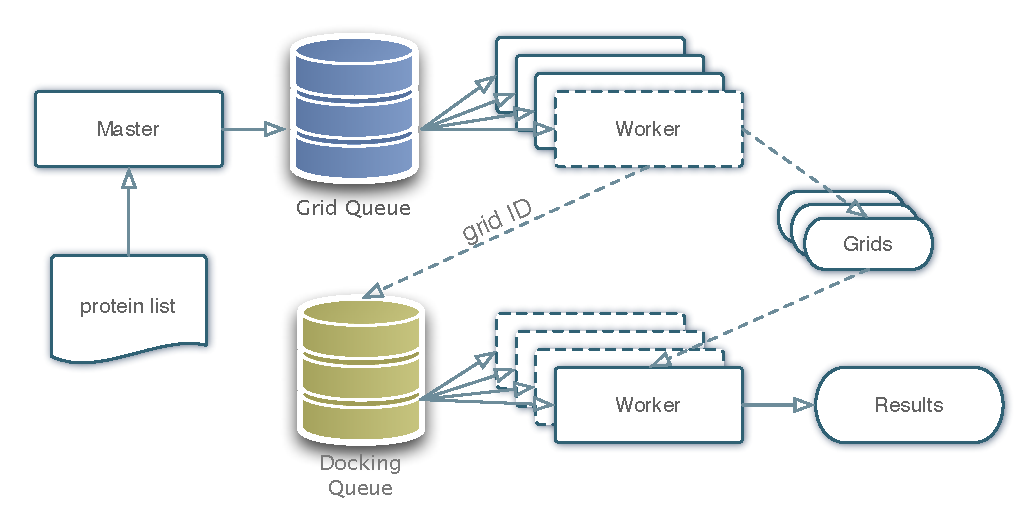
\includegraphics[width=0.85\linewidth]{images/Romain/fig3-color}
	\end{center}
	\caption{Représentation du flot d'exécution dans l'architecture distribuée}\label{fig:romain-fig3}
\end{figure}


\subsubsection{Optimisation aux clusters HPC}

 L'architecture distribuée présentée ci-dessous est adaptée à une exécution sur tout type de réseau d'ordinateurs (cluster, cloud, grille pervasive, etc.). Toutefois, il est possible d'optimiser son fonctionnement sur les clusters HPC si on prend en compte l'existence d'un gestionnaire de tâches propre à ces systèmes. En effet, la plupart des clusters HPC fait l'usage d'un gestionnaire de tâches afin de garantir la réservation et l'équité d'usage des ressources. Des systèmes tels que PBS, OAR ou Slurm sont capables de gérer plusieurs files d'exécution ainsi que de déployer des tâches en mode "best effort" de manière à occuper les ressources de calcul lorsque les réservations ne suffisent pas. 
 
 Dans le cas de l'optimisation pour les clusters HPC notre stratégie a été d'éliminer la dépendance à un noeud maître et permettre ainsi l'exécution des tâches indépendantes selon les disponibilités du gestionnaire de tâches. En effet, la présence d'un noeud maître était nécessaire afin de gérer les files d'exécution mais aussi de vérifier la terminaison des tâches (garantissant la tolérance aux fautes). Cela oblige donc que le processus maître reste actif pendant toute l'exécution, ce qui impose des problèmes lors de la réservation des ressources destinées au maître (combien de temps faut-il le garder actif ?). Cette limitation est encore plus importante dans le cas d'un déploiement best-effort, où la terminaison des tâches risque d'être fortement étalée au gré de l'occupation des ressources. Comme les gestionnaires de tâches des clusters HPC sont capables de détecter une tâche interrompue et la relancer, il suffit de soumettre dans une même tâche les paramètres nécessaires à la génération des sous-grilles et à leur docking. 
 
 Grâce à cette optimisation, l'outil AMIDE issu de ces travaux est capable d'effectuer le docking inversé autant dans un cluster géré que dans un agglomérat de machines indépendantes.
 
 \subsection{Évaluation pratique}
 
 Lors de la mise en place de l'outil AMIDE nous avons exécuté plusieurs expériences dans le but de valider notre approche de travail. L'un de ces tests consistait à évaluer la précision des stratégies de décomposition en étudiant un complexe ligand(X23)-protéine(3CM2) bien connu, autant par rapport à la technique classique du blind docking que par rapport à des données expérimentales obtenues par cristallographie. Dans un deuxième moment nous avons conduit des tests de performance, où le docking inverse était effectué sur un large ensemble de protéines issues de la bibliothèque PDB.
 
Toutes les expériences ont été conduites sur le cluster Clovis du centre de calcul ROMEO à Reims. Clovis était un cluster hybride avec 36 noeuds Westmere-EP (12 coeurs), 2 noeuds Nehalem-EX (32 coeurs), un noeud Westmere-EP (12 coeurs + 2 Fermi C2050 GPUs) et un noeud Nehalem-EP (8 coeurs + GPU Fermi M2090), et au moins 2GB de mémoire par coeur. Pour une question de régularité, les expériences ici présentées on été lancées exclusivement sur les noeuds Westmere-EP nodes. De plus, afin de mieux évaluer la communication intra-cluster, seulement 4 coeurs de calcul ont été utilisés par noeud.
 
 Ainsi, pour la première expérience, nous avons initialement exécuté un blind docking de la protéine 3CM2 et du ligand X23. Comme illustré en  Fig. \ref{fig:blind}, le blind docking a permis la détection de la cavité et d'une conformation presque identique à celle obtenue par cristallographie (différence RMSD de 1.60 Angstroms seulement).
 
 \begin{figure}[h]
 	\begin{center}
 		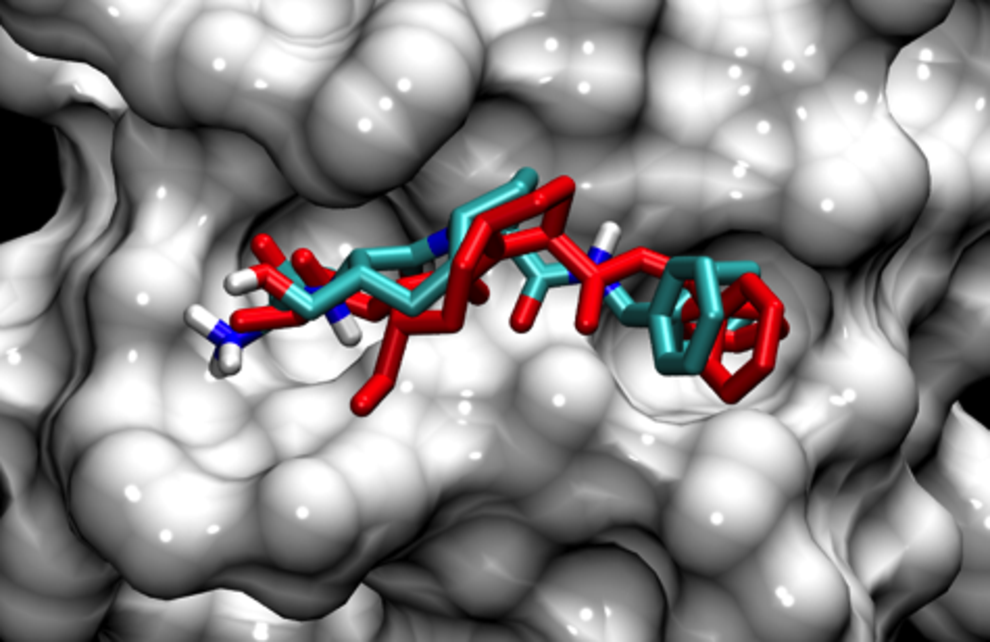
\includegraphics[width=1\linewidth]{images/Romain/fig4-color} 
 		\caption{Placement du ligand selon la méthode cristallographique (rouge) et celle obtenue par blind docking (vert)}\label{fig:blind}\vspace{-0.3cm}
 	\end{center}
 \end{figure}
 
 \begin{table}
 	\begin{center}
 		\caption{3CM2 docking accuracy of decomposing strategies with different number of runs. RMSD is compared to the experimental pose and binding energies are compared to those obtained by blind docking.}\label{tab:rmsd}
 		\begin{tabular}{|c|c|c|c|}
 			\hline 
 			$\Delta G$ blind docking & Number of runs  & $\Delta G$ cutting & RMSD  \\ 
 			($kcal.mol^{-1}$)  & for cutting method & ($kcal.mol^{-1}$) &  ($\AA$) \\
 			\hline 
 			\multirow{3}{*}{$\Delta G = -10.27$}  & 20 & $\Delta G_{12} = -10.09$ & 1.79 \\ \cline{2-4}
 			& 50 & $\Delta G_{pocket} = -10.11$ & 1.86 \\ \cline{2-4}
 			& 70 & $\Delta G_{pocket} = -10.39$ & 1.62 \\ \cline{2-4}
 			\hline 
 		\end{tabular} 
 	\end{center}
 	\vspace{-0.3cm}
 \end{table}
 
 The space cutting with the better free energy binding is $n = 12$, as illustrated in Fig. \ref{fig:cuts}. With only 20 docking runs, this type of decomposition gives the same free binding energy as the blind docking experiment and a RMSD pose of 1.79 Angstroms (see Table \ref{tab:rmsd}). Even if they succeed in replacing the ligand in the experimental cavity (as the blind docking), the other cuttings n = 8, 27 or 64, do not give satisfying results in term of binding energy and RMSD value.
 
 \begin{figure}[h]
 	\begin{center}
 		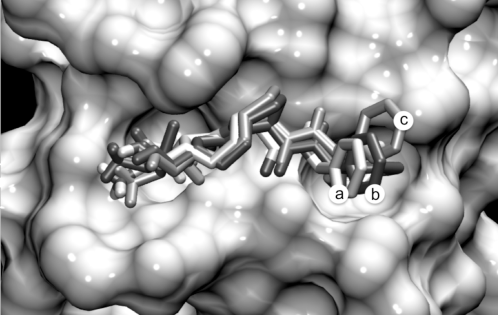
\includegraphics[width=1\linewidth]{images/Romain/fig5-bw} 
 		\caption{Ligand pose from the blind docking compared to methodology best results. X23 pose from the blind docking in light grey (a), X23 pose from the n = 12 cutting in dark grey (b) and X23 pose from the pockets search in medium grey (c).}\label{fig:cuts}\vspace{-0.3cm}
 	\end{center}
 \end{figure}
 
 It is important to highlight that the pocket search derived from \textit{Fpocket} experiment is able to predict the subspace and placing the ligand with $\Delta G = -10.11~kcal.mol^{-1}$ and a RMSD value of 1.86 Angstroms for a 50 runs docking experiment. 
 
 In a second experiment, we carried out a larger experiment in which we tested our ligand (X23) on a set of 100 proteins from the PDB. 
 Fig. \ref{fig:performance} compares the raw performance of the different techniques when the number of runs performed is proportional to the 3D box volume. Hence, if we consider that the space cutting respects the box proportions, the ideal number of runs for a cutting n = 8 without overlapping should be 256 / 8 = 32, for example. Not all decomposition techniques are prone to this proportional rule, for example the pocket strategy that targets cavities with variable dimensions. In this case, we present the computational cost for a fixed number of runs (50, for instance).  
 
 \begin{figure}
 	\begin{center}
 		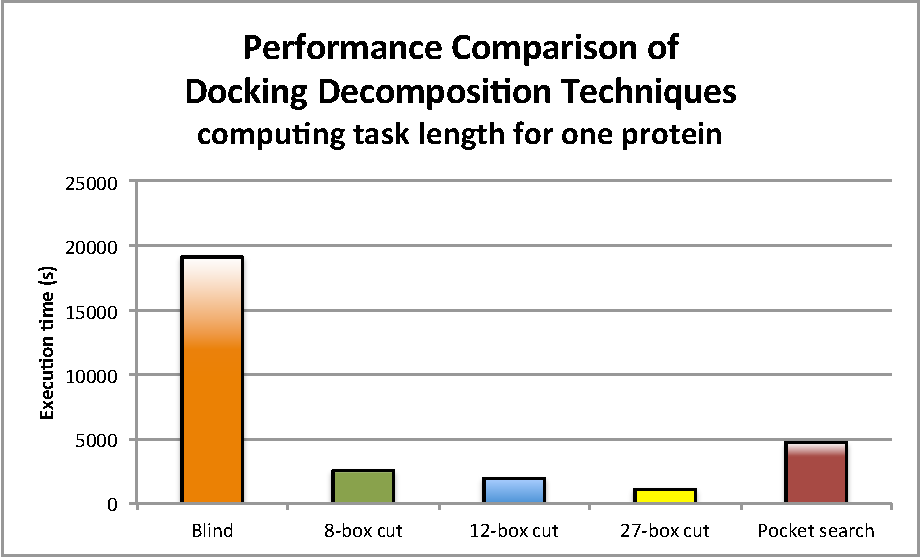
\includegraphics[width=0.8\linewidth]{images/Romain/fig7-color} \vspace{-0.3cm}
 		\caption{Performance comparison between different decomposition strategies for the 3CM2 protein.}\label{fig:performance}\vspace{-0.3cm}
 	\end{center}
 \end{figure}
 
 By using a proportional number of runs for the blind strategy and $n$=8, 12 and 27, we are able to conduct the same number of evaluations in less time, while improving distribution. Nonetheless, an indivisible preprocessing cost at the beginning of each docking execution prevents a linear acceleration, and it is also important to consider that the accuracy of the different techniques is not the same: as shown in the previous section, a strategy with a 12-part cutting with 21 runs is much more precise than a 8-part cutting with 32 runs due to the use of overlapping areas. We can point out that the cost for the pocket strategy also depends on the number of identified cavities and the size of the pocket box. In the case of the 3CM2 protein, only one cavity was identified but this number may be higher or cover a larger portion of the protein.
 
 In spite of the overall computational cost, the use of decomposition methods present clear advantages when regarding fault tolerance and load balancing. By dividing the docking of a protein in several tasks, we limit the losses in the case of a failure. For example, a computer failure in a blind docking that takes more than 5h30 requires the re-execution of the entire docking; this is not the case in a 12-part decomposition, where at most half-hour is lost. In addition, the use of a bag-of-tasks queue mechanism improves the load balancing, as illustrated in Fig. \ref{fig:balance}.
 
 In the case when all the available resources are less important than the number of tasks, computation time increases irremediably whatever the method employed. Nevertheless, we proved on a large set of proteins, that our method performed a better volume exploration and gave better results than the blind docking. In addition, we can better distribute the load, better manage the resources and improve fault-tolerance.
 
 \begin{figure}[h]
 	\begin{center}
 		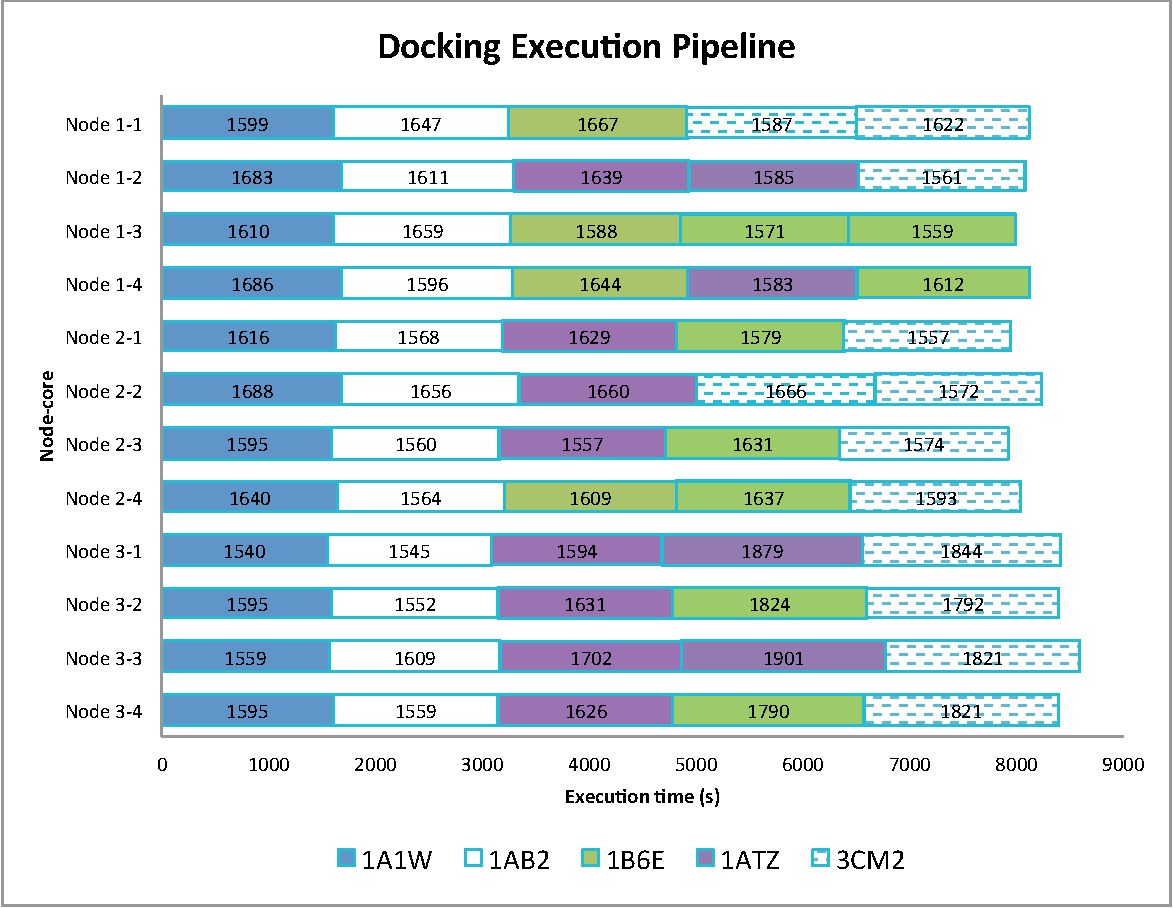
\includegraphics[width=0.75\linewidth]{images/Romain/fig8-color} 
 		\caption{Load balancing observed during a docking with 5 proteins (the individual task times are shown in the bars).}\label{fig:balance}\vspace{-0.5cm}
 	\end{center}
 \end{figure} 
 

\section{Hétérogénéité des Ressources de Calcul} \label{sec:intro}

Apache Hadoop is a popular framework for distributed and parallel computing. It implements the MapReduce programming paradigm, which aims at processing big datasets \cite{Dean2008} and to scale up from a single server to thousands of machines. 

Without specific configuration by the administrator, Apache Hadoop supposes the use of dedicated homogeneous clusters for executing MapReduce applications. As the overall performance depends on the task scheduling, Hadoop performance may be seriously impacted when running on heterogeneous and dynamic environments it was not designed for.   

This is a special concern when deploying Hadoop over pervasive grids. Pervasive grids are an interesting alternative to costly dedicated clusters, as the acquisition and maintenance of a dedicated cluster remain high and dissuasive for many organizations. According to \cite{Parashar2010}, pervasive grids represent the extreme generalization of the grid concept, in which the resources are pervasive. Pervasive grids use resources embedded in pervasive environments to perform computing tasks in a distributed way. Concretely, they can be seen as computing grids formed by existing resources (desktop machines, spare servers, etc.) that occasionally contribute to the computing grid power. These resources are inherently heterogeneous and potentially mobile, dynamically joining and leaving the grid. Knowing that, in essence, pervasive grids are heterogeneous, dynamic, shared and distributed environments, their efficient management becomes a very complex task~\cite{Nascimento}. Task scheduling is thus severely affected by the environment complexity.  

Many works proposed to improve the Hadoop framework on environments that diverge from the original working specifications (\cite{Kumar2012, Zaharia2008, Rasooli2012, Sandholm2010}). The PER-MARE project (\cite{PER-MARE}), in which this work was developed, aims at adapting Hadoop to pervasive environments \cite{3PGCIC}.

Therefore, adapting the execution to dynamic environments is a necessity as Hadoop is based on static configuration files that do not adapt to resources variations. Attempting install on heterogeneous clusters imply for the administrators to manually set the characteristics for each resource, a repetitive and time consuming task. All these factors prevent deploying Hadoop on more volatile environments, and our objective is to improve Hadoop so that it could adapt itself to the execution context and therefore be deployed over pervasive grids.

In order to adapt Hadoop to a pervasive grid environment, supporting context-awareness is essential. Context-awareness is the capacity of an application or software to detect and respond to environment changes \cite{Maamar}. A context-aware system is able to adapt its operations without human intervention, therefore improving the usability and efficiency of the system~\cite{Baldauf}. In pervasive grids, context-aware data may help task schedulers to make better decisions based on real feedback from the system.

This work focuses on our developments to introduce context-awareness capabilities on Hadoop task scheduling mechanisms. Through a context collection procedure and minimal changes on Hadoop's resource manager, we are able to update the information about the availability of resources in each node of the grid and then influence the scheduler tasks assignments. It also extends the preliminary observations from \cite{Cassales2015202} through the analysis of additional performance benchmarks.

The rest of the paper is organized as follows: Section \ref{sec:refteo} presents Apache Hadoop architecture and scheduling mechanisms. 
Section \ref{sec:related} discusses related work, focusing on context-awareness and on other works that try to improve Hadoop schedulers. 
Section \ref{sec:desenv} presents our proposal of context-aware scheduling, while Section \ref{sec:exper} presents the experiments conducted and the results achieved. Section \ref{sec:disc} introduces general discussion about the results and future challenges. We finally conclude this paper in Section \ref{sec:concl}.

\subsection{About Hadoop Scheduling} \label{sec:refteo}

Before discussing related works and presenting our proposal, it is worth introducing some basic concepts about the Hadoop framework and its schedulers. 

\subsubsection{Hadoop Framework Architecture}

The current Apache Hadoop framework is organized as a master and slave architecture, with two main services: storage (HDFS) and processing (YARN). Both services have their own master and slave components, as presented on Fig. \ref{fig:ArquiteturaHadoop}: the \textit{NameNode} and \textit{ResourceManager} services are the masters of the HDFS and YARN respectively, and the \textit{DataNode} and \textit{NodeManager} their slave counterparts. It is also possible to note the \textit{ApplicationMaster}, the component responsible for internal application management (task scheduling), while \textit{ResourceManager} is responsible for job scheduling. Each node also runs a set of \textit{Containers}, where the execution of Map and Reduce tasks takes place. 

\begin{figure}[!ht]
	\centering
	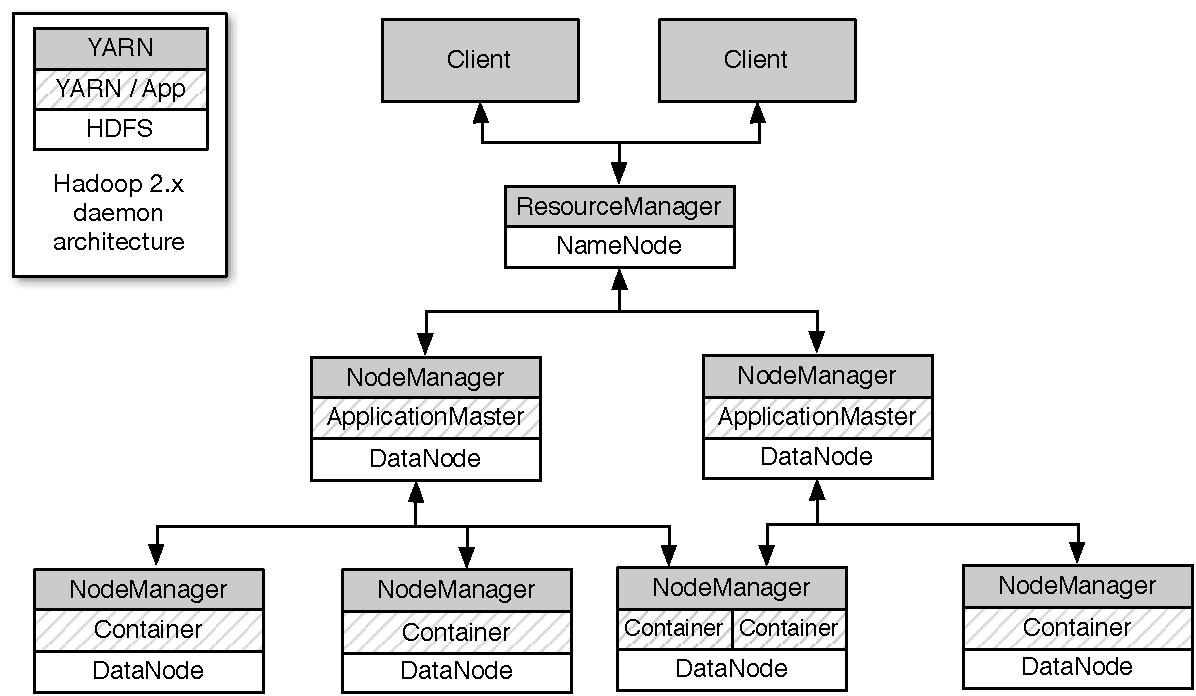
\includegraphics[width=1\linewidth]{img/HadoopArch.pdf}
	\caption{General Apache Hadoop architecture}
	\label{fig:ArquiteturaHadoop}
\end{figure}


\subsubsection{Hadoop Schedulers}

The Hadoop framework has two execution layers that depend on schedulers, according to their granularity. The coarse-grain instance is the job, while the fine-grain instance is represented by the tasks that compose a job. 

Job-level scheduling is performed by the \textit{ResourceManager}, an entity that has a global view of the available resources and can, for instance, arbitrate available resources among the competing applications. Each application is associated to an \textit{ApplicationMaster} that tries to acquire the right to use a given number of resource units (\textit{containers}) from the \textit{ResourceManager};  the latter must optimize the resources utilization according to different constraints such as capacity guarantees, fairness, and SLAs. 

 The \textit{ResourceManager} can be optimized to different constraints and parameters through the use of pluggable schedulers. The simplest scheduler algorithm, \textit{Internal Scheduler}, processes all jobs in the order of arrival (FIFO). This scheduler performs well in dedicated clusters where the competition for resources is not a problem. Another scheduler available is the \textit{Fair Scheduler}, which uses a two level scheduling to fairly distribute the resources among batches of small jobs \cite{Hadoop}. A third widely known scheduler is the \textit{Capacity Scheduler}, which is designed to run Hadoop MapReduce in a shared, multi-tenant cluster. The Capacity Scheduler is designed to allow sharing a large cluster while giving each organization a minimum capacity guarantee. The central idea is that the available resources in the Hadoop MapReduce cluster are partitioned among multiple organizations that collectively fund the cluster based on computing needs \cite{Hadoop}.

These schedulers allows a flexible management of the framework at the job level. Yet, the available schedulers neither detect nor react to the dynamicity and heterogeneity of the computing environment, a requirement for pervasive grids. Indeed, the design of Hadoop YARN passes on this responsibility to the \textit{Application Master}, which can better adapt to the application needs.

At a fine-grain, scheduling is performed by the \textit{ApplicationMaster} according to the number of tasks and assigned resources. There is almost no documentation on the default task scheduler, but we can assume that it implements a progressive filling approach where tasks are fed to all granted containers in one node before starting filling the next node. This behavior was experimentally observed in \cite{UBICOMM2014}. 

It is also worth noting that the \textit{ApplicationMaster} is not aware of the real execution context as it relies on the resources granted by the \textit{ResourceManager}, i.e., it has only a limited view on the computing platform. Modifying the \textit{ApplicationMaster} scheduling algorithms to consider real context-awareness requires changes on the \textit{ResourceManager} itself. After reviewing some related work on the next session, we will introduce our approach to bring context-awareness to Hadoop.


\subsection{Related Work} \label{sec:related}

Over the years, different works proposed improvements to the Hadoop scheduler mechanisms in order to respond to specific needs. These contributions may be classified as new scheduling methods or as improvements for the resource distribution.

Works like \cite{Kumar2012}, \cite{Tian2009} and \cite{Rasooli2012} assume that most applications are periodic and demand similar resources regarding CPU, memory, network and hard disk load. These assumptions allow the applications and nodes to be analyzed regarding the CPU and I/O potential, enabling the optimization of  execution through matching of nodes and applications with the same characteristics. \cite{Isard2009} focus on a new scheduling method proposing the usage of a capacity-demand graph that assists the calculation of optimal scheduling based on an overall cost function.

While previous works focus on performance improvement using static information about resources and applications, other works sought to incorporate task specific information into their proposals. For example, \cite{Zaharia2008} and \cite{Chen} attempted to improve tasks distribution as a way to reduce the response time in large clusters. \cite{Zaharia2008} use heuristics to infer the estimated task progress and to make a decision about the launching of speculative tasks. Speculative tasks are launched when there is a possibility that the original task is on a node either faulty or too slow node. Another work (\cite{Chen}) proposes the use of historical execution data to improve decision making. 

Both scheduling mechanics and resource distribution methods result in a load rebalancing, forcing faster nodes to process more data and slower nodes to process less data. \cite{Sandholm2010} try to achieve that through a system based on resource supply and demand, allowing each user to directly influence scheduling through spending rates. The main objective is to allow a dynamic resource sharing based on preferences set by each user. 

There are also works such as \cite{Xie2010}, which attempt to provide a performance boost in jobs through better data placement, mainly using data location as information to decision making. The performance gain is achieved through data rebalancing on nodes, increasing the load on faster nodes. This proposal reduces the number of speculative tasks and data transfers over the network. A similar proposal is observed by \cite{Cavallo2015}, which address scheduling and data distribution issues on geographically distributed clusters. These authors present a new hierarchical scheduling mechanism based mainly on throughput and application data profiling. As for \cite{Xie2010}, \cite{Cavallo2015} also focus on optimizing data transfer through the network.     

\cite{Marozzo2012} uses a P2P structure to arrange the cluster. In this approach, nodes can change their function (master/slave) over time and can have both functions at the same time, the functions being tied to the applications and not to the cluster. The objective of this work is the adaptation of MapReduce paradigm to a P2P environment, which given the natural volatility of P2P environments, would offer support to pervasive grids. However, this proposal focuses on providing a resilient infrastructure and does not explore the scheduling of jobs and tasks. Another work relying on a P2P overlay, \cite{Steffenel20151034} offers MapReduce-like computing for pervasive environments on top of a general distributed computing platform. However, this platform focuses on fault-tolerance and volatility aspects through a fully distributed task scheduling mechanism, which for the moment does not implement context-aware scheduling optimizations.

Indeed, most of previously cited works do not actually consider the evolving state of the available resources. Resources are described, not observed. However, works on context-aware computing (\cite{Baldauf, Maamar, Ramakrishnan2014, Najar2015}) have demonstrated that this observation is possible and that the execution environment may influence application behavior. This raises a question: can we improve MapReduce scheduling by observing current execution environment? The next sections will try to answer this question.   

\subsection{Context-Aware Scheduling} \label{sec:desenv}
The main goal of this work is to improve the scheduling of Hadoop by adding support to dynamic changes at the \textit{Resource Manager} level. Unlike the works on Section \ref{sec:related} we opted to feed dynamic context information to an existing scheduler (\textit{Capacity Scheduler}) and therefore modifying the Hadoop source code the least possible. 

In the default Hadoop implementation, a \textit{NodeManager} declares its computing resources to the \textit{ResourceManager} when joining the Hadoop network, this information being usually obtained from static configuration files. In order to detect dynamic changes, the scheduler must collect context information that, in this case, refer to available resources on the nodes. Then, a \textit{NodeManager} communicates periodically with the \textit{ResourceManager} in order to keep information updated and let the scheduler adapt to the new context. In the following section we present a more detailed explanation of the changes implemented in Apache Hadoop.

\subsubsection*{Context collector}
By default, Hadoop reads information about the nodes from XML configuration files. These files contain many configuration parameters, including the resource capacity of each node. Once loaded, the information will not be updated until the service is restarted. As pervasive environments may face performance changes during the execution of an application, we need a mechanism that collects contextual information at runtime and subsequently updates the \textit{ResourceManager} knowledge base.

Therefore, we integrate into Hadoop a collector module, allowing to observe contextual information about the available resources. The collector was developed for the PER-MARE project \cite{PER-MARE}, and its class diagram is presented in Fig. \ref{fig:CollectorDiag} \cite{UBICOMM2014}. 
The collector module is based on the standard Java monitoring API (\cite{Oracle}), which allows to easily access the real characteristics of a node. It allows collecting different context information such as the number of processors (cores) and the system memory using a set of interface and abstract/concrete classes that generalize the collecting process. Due to its design, it is easy to integrate new collectors and improve the resources available for the scheduling process, providing data about the CPU load or disk usage, for example.

\begin{figure}[!ht]
	\centering
	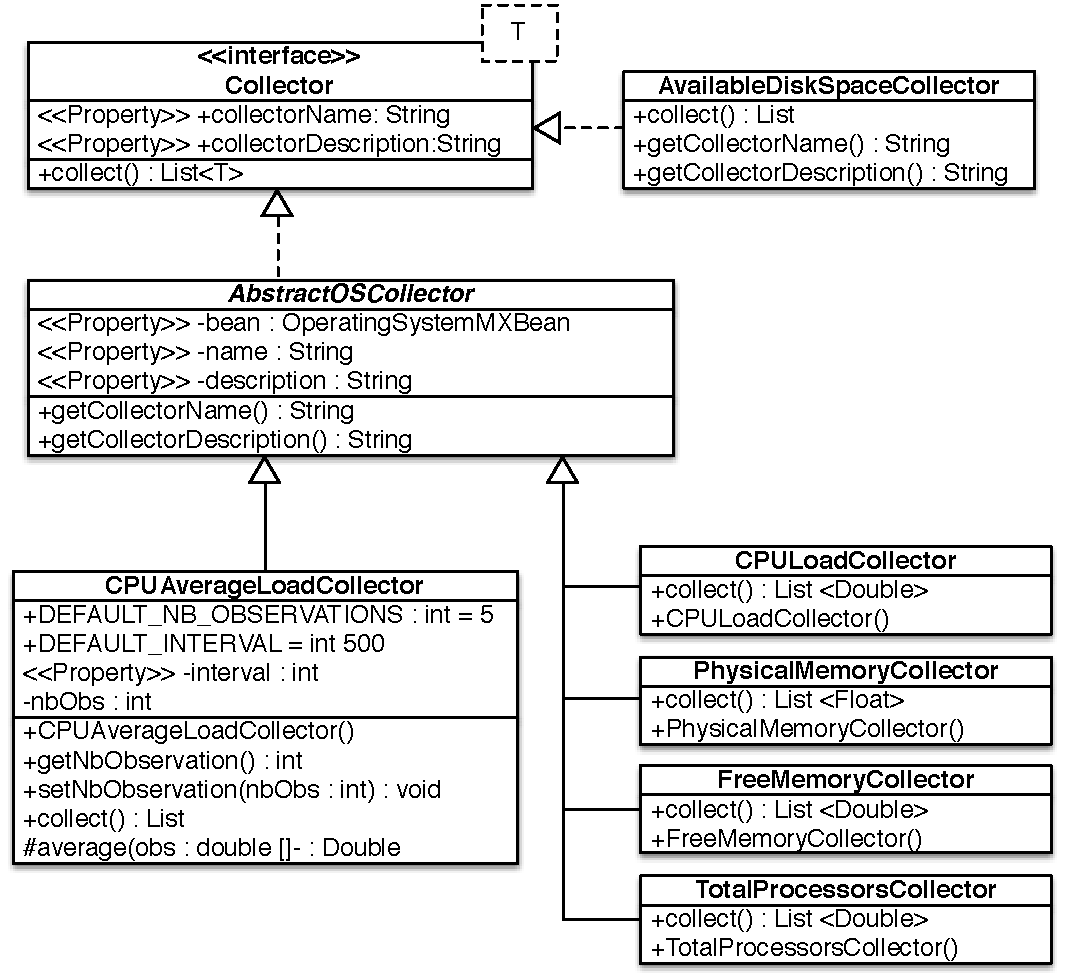
\includegraphics[width=1\linewidth]{img/CollectorUML2.pdf}
	\caption{Context collector structure}
	\label{fig:CollectorDiag}
\end{figure}

Nevertheless, replacing XML configuration files by the context collector is not enough, since a global knowledge of the available resources is necessary in order to adapt scheduling to runtime conditions. Indeed, to allow \textit{ResourceManager} to adapt scheduling to the current available resources, the context collector associated to each node must be able to communicate its current state to the \textit{ResourceManager} during the execution. In order to do so, we have improved communication capabilities of both \textit{ResourceManager} and \textit{NodeManager} as explained in the following section.    

\subsubsection*{Communication}
Gathering the context information requires to feed the Hadoop scheduler requires transmitting this information through the network from slave nodes (\textit{NodeManager}) to the master node (\textit{ResourceManager}) which is in charge of the scheduling. Instead of relying on a separate service, we chose to use the ZooKeeper API \cite{Hunt2010} that provides efficient, reliable, and fault-tolerant tools for the coordination of distributed systems. In our case, ZooKeeper services are used to distribute context information. 

\begin{figure}
	\centering
	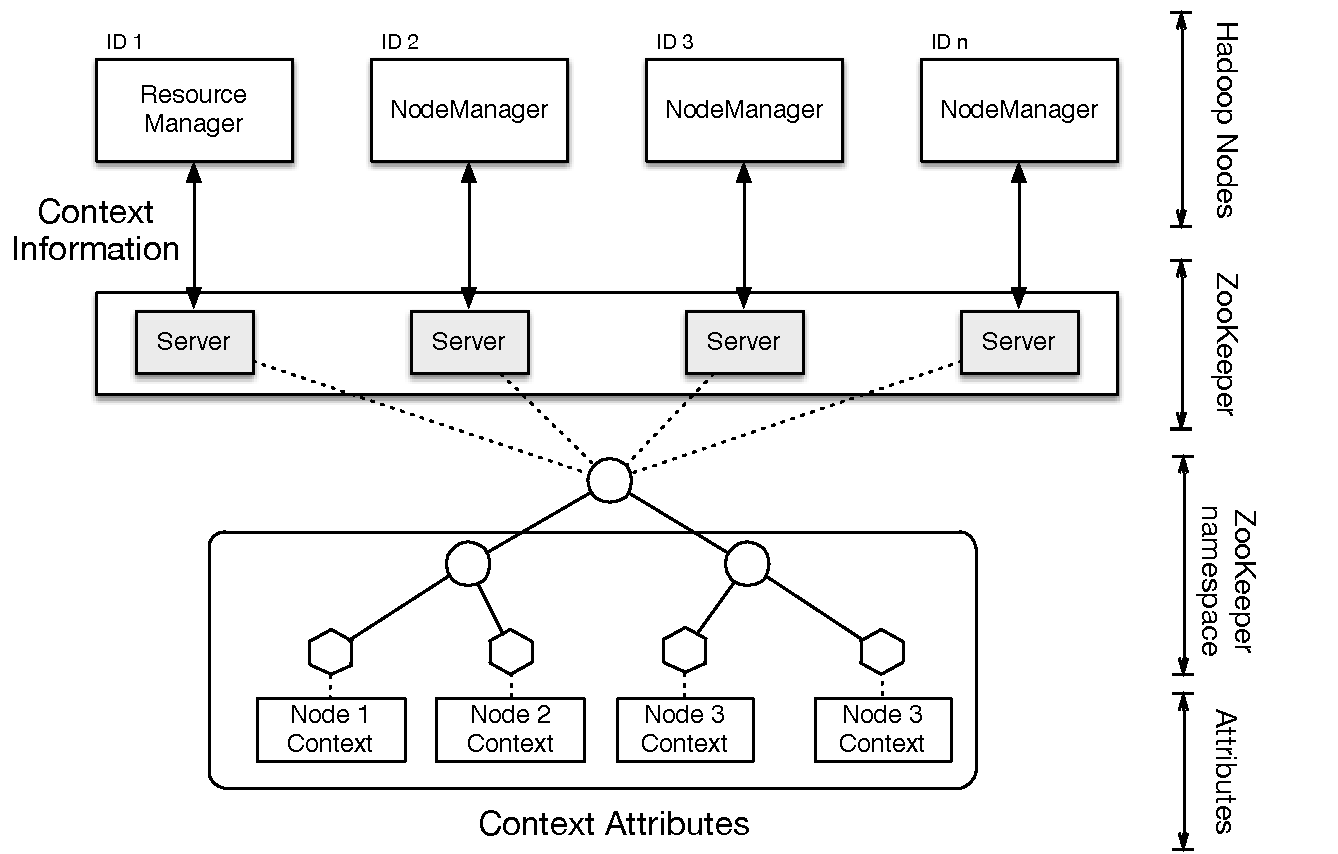
\includegraphics[width=1\linewidth]{img/Zookeeper} 
	\caption{Using ZooKeeper to distribute context information\label{fig:zookeeper}}
\end{figure}


As illustrated in Fig. \ref{fig:zookeeper}, all slaves (\textit{NodeManager}) run an instance of the \textit{NodeStatusUpdater} service, which collects data about the real resources availability (for example, every 30 seconds). If the amount of available resources changes, the DHT on ZooKeeper will be updated. Since the Operating System produces some variations on the resources, this information will only be changed if the variation is big enough to raise/lower the maximum capacity of containers on that node. This small change will spare a lot of executions where the information changed, but the variation was not enough to impact the scheduling. Similarly, the master (\textit{ResourceManager}) also creates a service to watch ZooKeeper's zNodes. If the Zookeeper node detects a DHT change, the master will be notified and will update the scheduler information based on the new information. This solution extends a previous one presented in \cite{UBICOMM2014} by offering a real time observation of available nodes. Indeed, our previous solution only updates information regarding the resources on service initialization, replacing the XML configuration file, while this one updates resource information whenever the availability changes. As a result, scheduling is performed based on the current resource state.


\subsection{Experiments and Results} \label{sec:exper}

In order to evaluate the impact of context awareness on the job scheduler mechanism, we performed two sets of experiments. In the first one, presented on Sections \ref{sec:5.3} and \ref{sec:5.4}, we considered a small dedicated cluster so that the stress of incorrect resources estimation could easily be controlled and analyzed. On the second set of experiences, presented on Sections \ref{sec:5.5} and \ref{sec:5.6}, we run the TeraSort benchmark in a larger number of nodes but a real shared environment (i.e., with nodes shared with other users and applications). Both the first and the second experiments considered different execution scenarios as well as different application profiles, as presented in the following section. 

\subsubsection{Execution scenarios\label{sec:scenarios}}

In the context of this work we compare the Hadoop behavior under different execution scenarios using the available memory and the number of nodes (\textit{v-cores}) as resource metrics. These parameters are reported to the \textit{ResourceManager} and represent the main elements considered by the Capacity Scheduler algorithm. In addition, the available memory parameter can  be considered as closely related to the node real environment (contrarily to the \textit{v-cores}) and is easily configurable through the \textit{yarn.nodemanager.resource.memory-mb} property. 

The execution scenarios were tailored to reproduce different combinations of reported resources, available resources and context awareness. Indeed, the execution performance is closely related to the assignment of computing resources to the applications. Incorrect configuration parameters or external factors may heavily impact the nodes performance, especially when these parameters lead to the resources overload. Similarly, changes on the available resources during the execution may drive a well-configured environment to an overloaded state if the changes are not reported to the scheduler. The four scenarios described below try to reproduce these situations, thus providing sufficient information for the analysis and discussions at the end of this paper. 

\textbf{Scenario A:} in this scenario we simulate a dedicated Hadoop cluster so that the reported memory always correspond to the available memory, which can be considered as the "best case" scenario. We consider the reported memory as the information that the scheduler use in the scheduling process, while available memory is the free memory of the node or cluster. Using a direct notation, the reported memory is 100\% and the available memory is also 100\% all through the execution.

\textbf{Scenario B:} in this case nodes can be used for other purposes than running Hadoop, so the reported memory may at some point differ from the available memory initially configured for Hadoop usage. This case corresponds to the default behavior of Hadoop, where memory resources are provided through a property \textit{yarn.nodemanager.resource.memory-mb}. Because the scheduler never adapts to the reduced resources, we consider it the "worst case" scenario. On this scenario, using a direct notation, the reported memory is 100\%, but the available memory is 50\%. 

\textbf{Scenario C:} in this case, the nodes are shared with other applications (like in Scenario B) but the context-awareness collector is active, updating context information every 30 seconds. When the MapReduce application is launched, the scheduler is aware of the execution context and can assign tasks according to the available resources. Using a direct notation, the reported memory and the available memory correspond to 50\% of the values reported on Scenario A.

\textbf{Scenario D:} this scenario presents an extension of Scenario C where the MapReduce application starts before the context collector update. The scheduler starts with wrong available resource information and must therefore adapt during the execution with the help of the context collector. Using a direct notation, the reported memory at the beginning of the execution is 100\% of the resources from Scenario A (wrong information), but at runtime this information is updated to 50\%. 

Scenario A corresponds to the "best case" for Hadoop framework, in which all resources are available during the entire execution. Scenario B simulates Hadoop execution in a heterogeneous environment where resources fluctuate during the execution but the scheduler is never aware of the changes (a "worst case"). If we consider context information, Scenario C illustrates a situation in which the context collector is able to detect environment changes before application execution starts while scenario D suffers from late information update but can still adapt to the changes. These two scenarios allow us to evaluate the impact of the context-aware scheduler during the deployment of an application in a heterogeneous environment.   

\subsubsection{Application benchmarks}

While big-data applications are expected to rely on memory, other factors like CPU usage and I/O may also impact the execution of the applications. For this reason, this work uses three different benchmarks, each characterized by different memory, CPU and I/O usages \cite{Benchmarks}. The three benchmarks are the following:
\begin{itemize}
	\item TeraSort: The goal of TeraSort benchmark \cite{TeraSort2008} is to sort a given amount of data as fast as possible. It is a benchmark that combines testing the HDFS and MapReduce layers of a Hadoop cluster. Because of the sorting algorithms, this benchmark stress memory and CPU;
	\item WordCount: the WordCount benchmark is the basic MapReduce example. Its objective is to count the number of occurrences of each word in a given text. Because WordCount memory and I/O usage are limited (both memory and output structures are small in comparison to the input file), the main performance is notably determined by the CPU;  
	\item TestDFSIO: The TestDFSIO benchmark is a read and write test for HDFS. It is helpful for tasks such as stress testing HDFS, to discover performance bottlenecks in the network, OS and Hadoop setup; it aims at giving a first impression of how fast a cluster is in terms of I/O. Memory and CPU are less solicited.
\end{itemize}

For the experiments we use the HiBench benchmarks suite, which is detailed in \cite{HiBench}. The TeraSort benchmark was run using a data set of 15 GB, TestDFSIO was run with 90 files of 250 MB and WordCount used a 10 GB file as input. 

\subsubsection{Environment setup and configuration for the controlled experiments\label{sec:5.3}} 
  
In order to test the new behavior of the framework, we conducted experiments with the Grid'5000 platform \cite{g5k}. We configured a dedicated network with 4 slaves, each having the following configuration: 2 Intel Xeon CPU E5420 @ 2.50 GHz (totalizing 8 cores per node) and 8 GB of RAM. All nodes run Ubuntu-x64-12.04, with JDK 1.7 installed, and the Apache Hadoop 2.5.1 distribution.

The resources evaluated in the experiments were the memory and number of cores, which have a direct impact on the amount of Map tasks allocated. In addition to the overall performance of each benchmark on the different scenarios, we performed an in-depth investigation on the tasks (containers) distribution throughout the execution. The information about the execution of each container was obtained from the Hadoop logs. These information allow us to present detailed Gantt charts of the tasks placement during the experiments.

To emulate the scenarios with reduced resources (Scenarios B, C and D), we opted to halve the number of nodes while reporting the same amount of global available memory as in Scenario A. While this approach is unrealistic (resources from failing nodes should be withdrawn from the available resources set), it provides a clear reference for the analysis of the scheduler decisions. 


\subsubsection*{Results from the controlled experiments\label{sec:5.4}} 


The results from experiments are presented in both  Tables \ref{tab:resumo}, \ref{tab:DFSIO}, \ref{tab:WC} and Figures \ref{fig:gantts}, \ref{fig:DFSIO}, \ref{fig:WC}, respectively for TeraSort, TestDFSIO and WordCount. All Tables summarize the experiments presenting the total time used by all map tasks, the average execution time, the standard deviation  and the number of speculative tasks launched on each scenario and for each benchmark. 

\begin{table}[h!]
	\caption{Summary of TeraSort results expressed in seconds.} \label{tab:resumo}
	\begin{tabular*}{\hsize}{lllll} 
		\textbf{Scenario} & \textbf{A} & \textbf{B} & \textbf{C} & \textbf{D}\\
		\hline
		Total Map Time ({\it{s}}) & 149 & 788 & 348 & 477 \\
		Avg. Map Time ({\it{s}}) & 39.47 & 222.97 & 38.38 & 68.42 \\
		Standard Deviation & 15.73 & 59.86 & 18.09 & 29.91 \\
		\# Map Tasks & 76 & 76 & 76 & 76 \\
		\# Speculative Tasks & 2 & 1 & 3 & 1 \\
	\end{tabular*}
\end{table}

\begin{table}[h!]
	\caption{Summary of TestDFSIO results expressed in seconds.} \label{tab:DFSIO}
	\begin{tabular*}{\hsize}{lllll} 
		\textbf{Scenario} & \textbf{A} & \textbf{B} & \textbf{C} & \textbf{D}\\
		\hline
		Total Map Time ({\it{s}}) & 139 & 444 & 239 & 364 \\
		Avg. Map Time ({\it{s}}) & 38.95 & 85.01 & 32.20 & 81.62 \\
		Standard Deviation & 17.20 & 69.08 & 8.30 & 73.60 \\
		\# Map Tasks & 90 & 90 & 90 & 90 \\
		\# Speculative Tasks & 0 & 9 & 0 & 1 \\
	\end{tabular*}
\end{table}


\begin{table}[h!]
	\caption{Summary of WordCount results expressed in seconds.} \label{tab:WC}
	\begin{tabular*}{\hsize}{lllll}
		\textbf{Scenario} & \textbf{A} & \textbf{B} & \textbf{C} & \textbf{D}\\
		\hline
		Total Map Time ({\it{s}}) & 155 & 1009 & 309 & 805 \\
		Avg. Map Time ({\it{s}}) & 43.76 & 208.39 & 41.73 & 175.80 \\
		Standard Deviation & 15.61 & 128.90 & 10.99 & 151.59 \\
		\# Map Tasks & 90 & 90 & 90 & 90 \\
		\# Speculative Tasks & 1 & 15 & 1 & 10 \\
	\end{tabular*}
\end{table}

Figures \ref{fig:gantts}, \ref{fig:DFSIO} and \ref{fig:WC} present the Gantt charts for each benchmark and scenario. For a given benchmark, each scenario is composed by either 2 or 4 lines, one for each node in the cluster during the experiment. As stated in the description of the scenarios, Scenarios B, C and D run on half of the nodes in Scenario A to simulate a reduced amount of resources. On each line we consolidate the resources according to a color scale where the darker the tone, the more containers run simultaneously and thus, more overloaded the node is. For instance, white means no container executing, and black means 16 containers. Additionally, the lines are segmented along the chart to indicate that a container has either finished or started at that moment. The charts are  scaled in seconds and all charts for a given benchmark have the same scale. Hence, TeraSort charts go from 0 to 790 seconds, TestDFSIO go from 0 to 450 seconds and WordCount from 0 to 1010 seconds.

While the Gantt charts represent the tasks (containers) execution, some containers are not affected by scheduling, such as the \textit{ApplicationMaster} or the Reduce tasks. For this reason, we ignore these tasks and concentrate the analysis on the elements that can be affected by the context-aware scheduling.

\begin{figure*}[!ht]
	\centering
	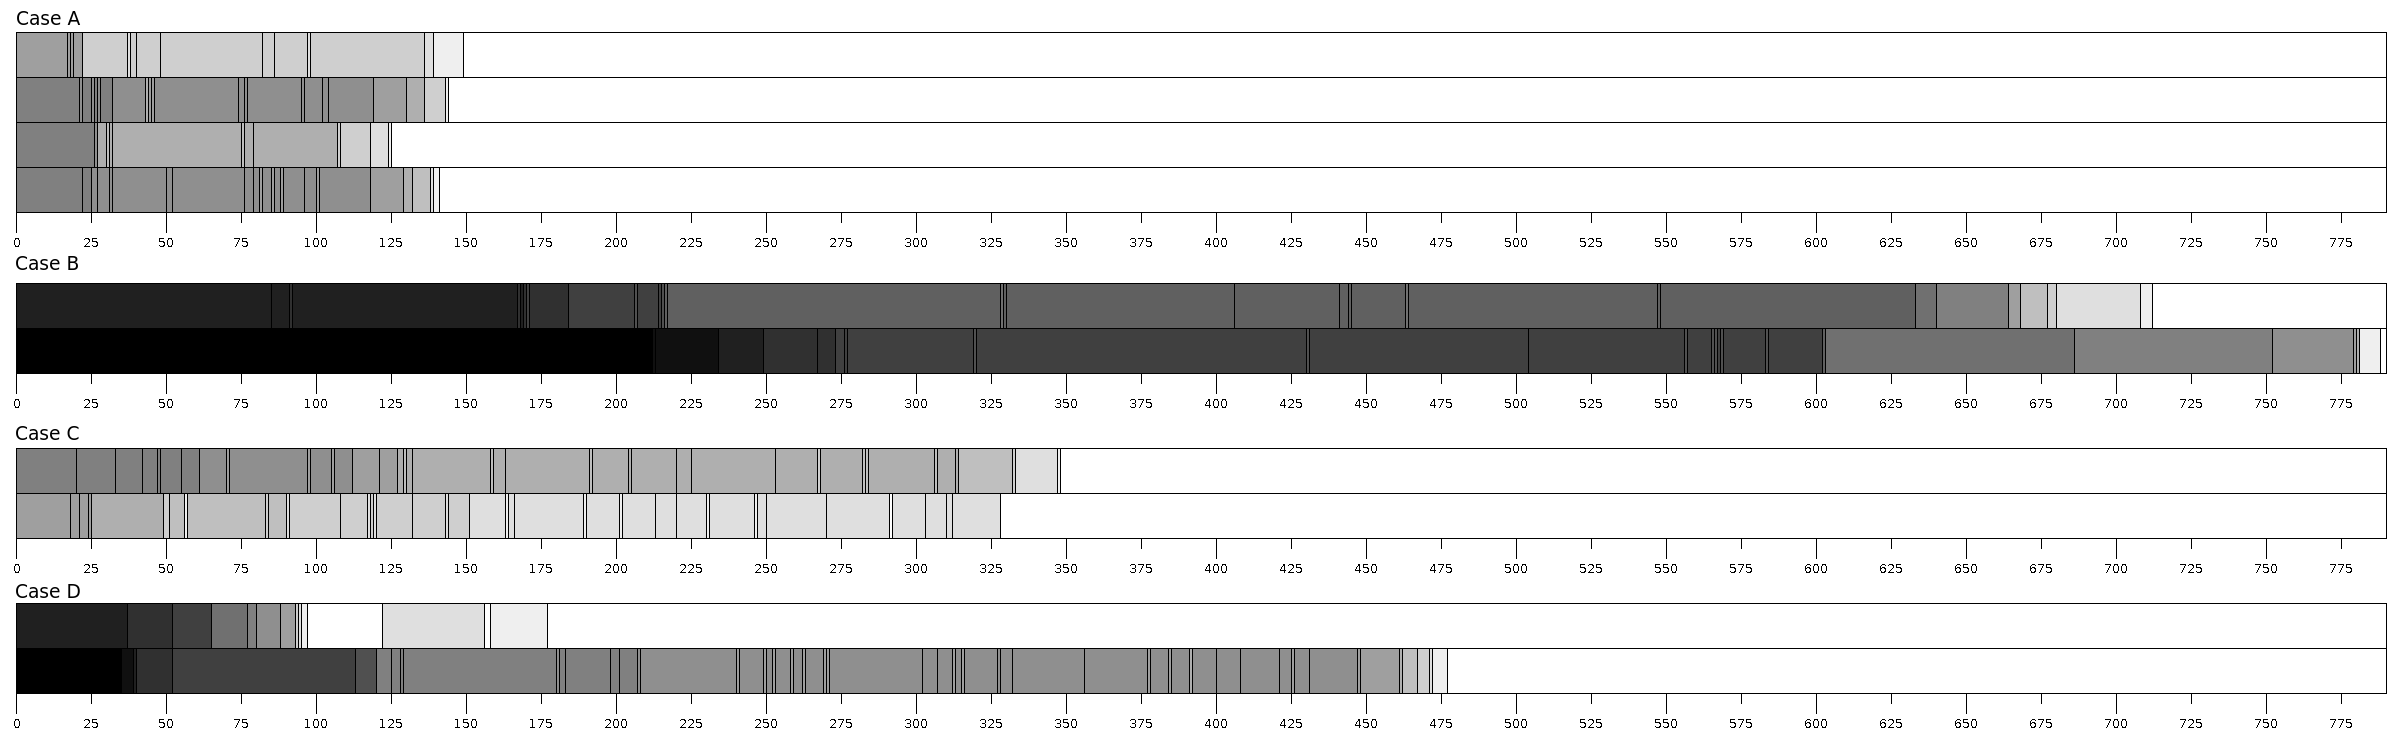
\includegraphics[width=1\textwidth]{img/todos}
	\caption{Gantt charts of the TeraSort experiments}
	\label{fig:gantts}
\end{figure*}

\begin{figure*}[!ht]
	\centering
	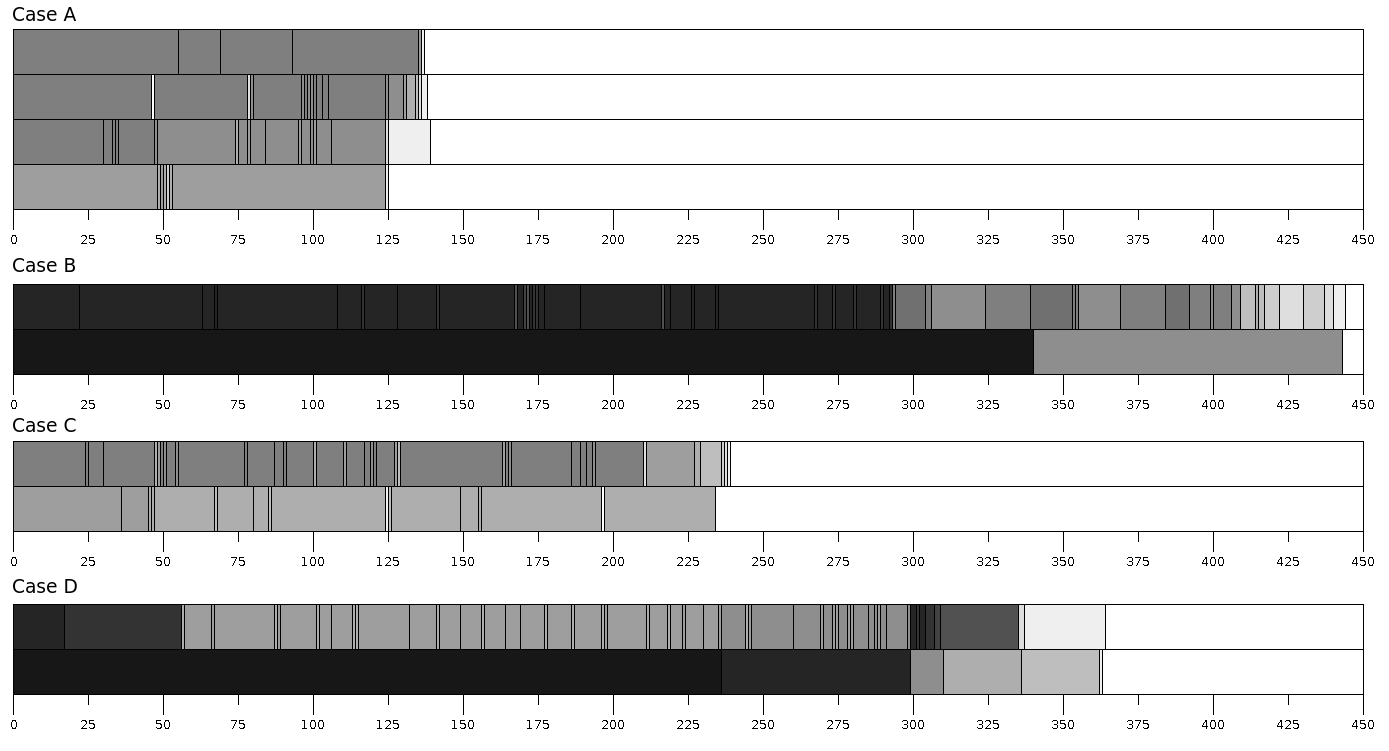
\includegraphics[width=1\textwidth]{img/todos-DFSIO}
	\caption{Gantt charts of the TestDFSIO experiments}
	\label{fig:DFSIO}
\end{figure*}

\begin{figure*}[!ht]
	\centering
	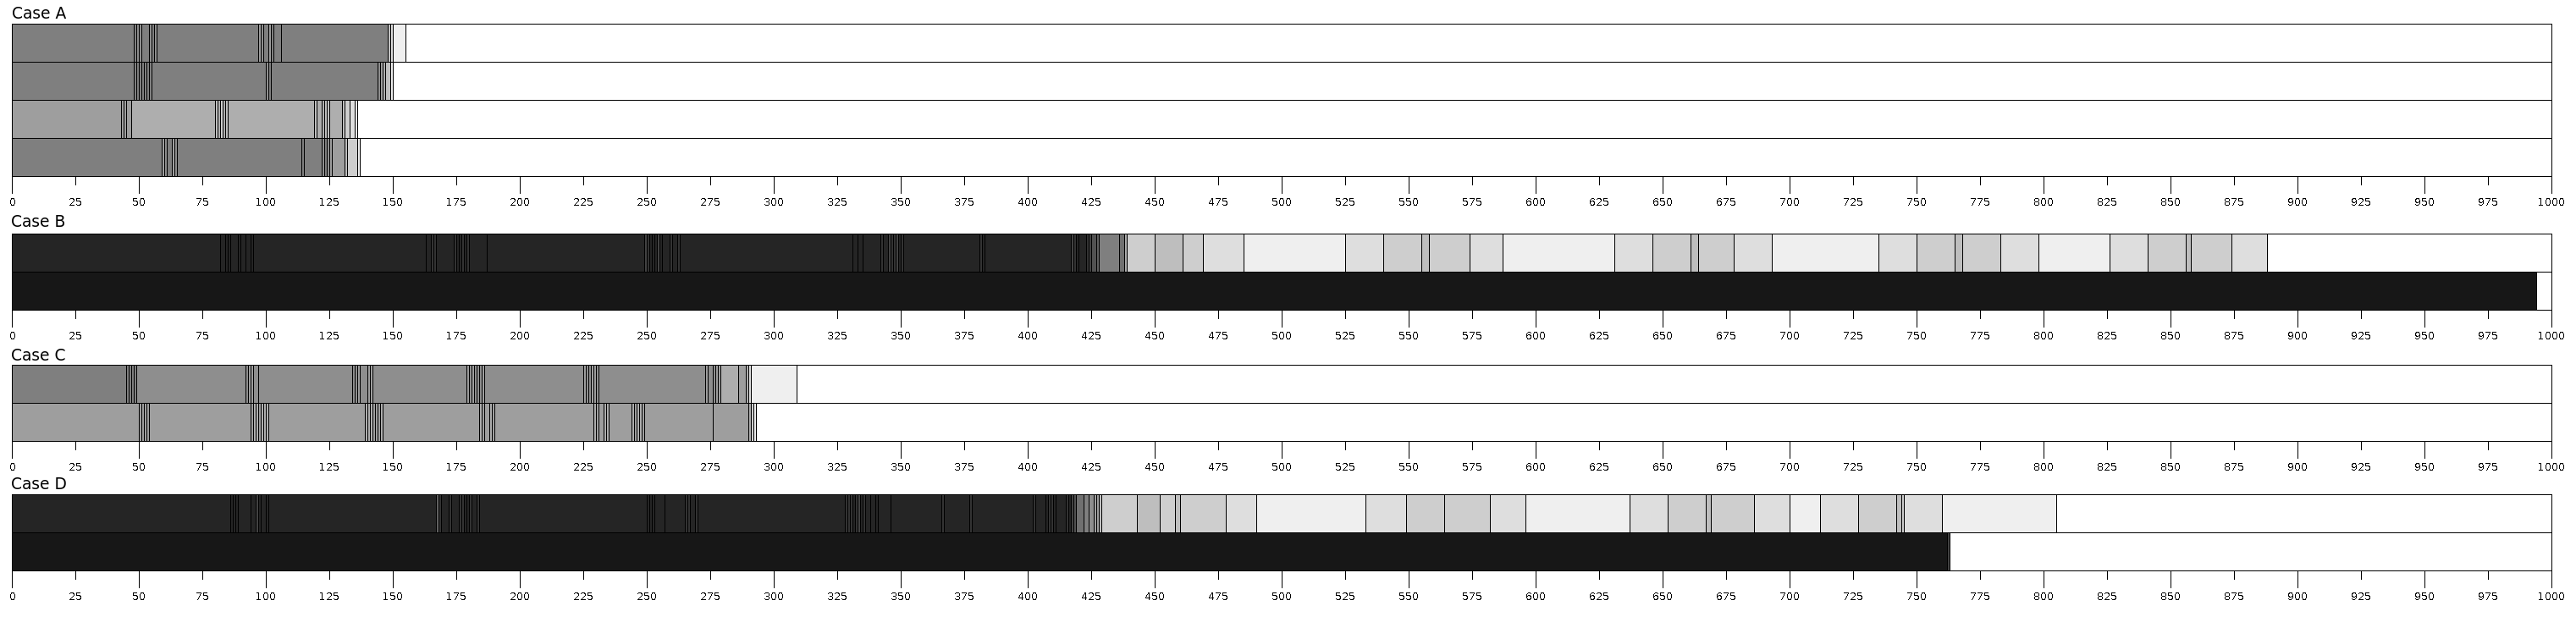
\includegraphics[width=1\textwidth]{img/todos-WC}
	\caption{Gantt charts of the WordCount experiments}
	\label{fig:WC}
\end{figure*}

From the analysis of the Tables, it is possible to identify some common trends. Indeed, all experiments present a similar behavior when we consider the Total Map Time: case A was the fastest, followed by C, D, and finally B. In addition, scenarios A and C showed not only the smallest Average Map Times and Standard Deviations among their applications, but also very similar results in these categories, regardless the benchmark. This is due to the fact that the nodes were never overloaded since the scheduler had an updated information before the start of the application. The charts also corroborate this analysis: in all experiments, cases A and C have much lighter tones than the others, meaning that less containers are running simultaneously. It is also worth noting that case C takes approximately twice the time case A used to complete the execution, a result to be expected since case C had half the resources of case A. 

The analysis of the number of speculative tasks also gives interesting insights. In the case of TeraSort, the number of speculative tasks is reduced and almost similar in all scenarios. TestDFSIO and WordCount, on the other hand, deploy many more speculative tasks when the system is overloaded (scenarios B and D). This may be due to the factors that trigger a speculative task: a speculative task is launched only after all the tasks for a job have been launched, and then only for tasks that have been running for some time (at least a minute) and have failed to make as much progress, on average, as the other tasks from the job. In the case of TeraSort, tasks evenly require both memory, CPU and I/O, so their execution time is less subject to specific resource depletion. TestDFSIO and WordCount, on the contrary, rely on more specific resources and thus are more subject to resource overload. In all the cases, the use of context-awareness on scenario D helps minimizing the number of speculative tasks when comparing to the "context-unaware" scenario B.

Concerning the execution flow, as illustrated by the Gantt charts, it is possible to note that both cases B and D have a dark tone at the beginning, meaning that 16 containers are running (twice the real capacity). Also, the first containers took 20 to 50 seconds to complete execution in scenarios A and C in all experiments (cf. the first segment line). On the opposite side, during most of scenario B (and to a lesser extent D) 70 or more seconds are required, evidencing an overload on the nodes. The exception here is the TestDFSIO scenarios B and D, which have segment lines at about 25 seconds. Through further analysis, it is possible to note that all TestDFSIO experiments had at least one segment line near the 25 seconds mark, meaning this was a task very easily processed and somehow not affected by the node overload.

Although both B and D scenarios had the same initial conditions (50\% available resources and 100\% reported resources), case D took less time to complete in all experiments (20\% to 40\% faster than B). The reason for this is that the context collector updates the reported resources in D, allowing the scheduler to reorganize tasks after the first tasks complete. This behavior is easily noted on TeraSort and TestDFSIO charts. Indeed, all D scenarios had high concentration of executing containers at the start of the job but lessened the load over time, while B scenarios had the nodes overloaded until the end due to the absence of updated information. Although the scheduler does not preempt excess containers, it is possible to observe a performance improvement of about 40\% on TeraSort and 20\% on TestDFSIO experiments as the scheduler avoids overloading the nodes.

There are some specificities that might be pointed out to better understand the charts. On all benchmarks, the first node is seemingly less charged in scenarios B and D after the initial executions. This is mostly due to the fact that after the initial computations this node hosts the Reduce containers, which were not included in the chart. It is important to remember that reducer tasks may start before the end of map tasks and that a reducer may even complete before all maps have finished processing. 

Although other specificities about the characteristics of the proposed jobs can be discussed, scenarios C and D show that regular context updates contribute to reduce the execution time on a dynamic Hadoop cluster. We demonstrated that even when starting with the same circumstances as in the worst case (Scenario B), updating the information helps the scheduler to minimize the execution time. Our solution contributes therefore to both provide correct information before the execution starts (Scenario C) and adapt the execution to resources changes (Scenario D). 

\subsubsection*{Environment setup for the shared execution environment\label{sec:5.5}}

As stated previously, this second set of experiments considered a more realistic environment, where we use 10 slave nodes in which part of the nodes are shared with another user. Indeed, most resource management systems (Slurm, Grid'5000 OAR) allow users to reserve only part of a node (for example, 8 from 16 cores). As the resources are not always evenly shared and some applications don't respect the limits from the allocated resources, this makes an interesting environment for the context-aware scheduler. Also, by increasing the number of slaves nodes, we aim to acquire more data about the solution scalability. 

Hence, this second environment presents a Scenario A with fully dedicated nodes, while in Scenarios B, C and D the first half of the nodes are shared. more exactly, each node has a total of 8 GB of memory and 8 cores but in a shared node only 2 GB  and 2 cores are available for Hadoop (the remaining 3/4 of the resources are assigned to another user). 

\subsubsection*{Results from shared environment experiments\label{sec:5.6}}


The results from the TeraSort benchmark on this shared environment is presented in Table \ref{tab:exp2} and Figure \ref{fig:exp2}. Once again, we compared the scheduler behavior under four different Scenarios: A, B, C and D, as described in Section \ref{sec:scenarios}. Table \ref{tab:exp2} summarizes the experiments, presenting the total time used by all map tasks, the average execution time, the number of successful map tasks and the number of speculative tasks launched. 

\begin{table}[h]
	\caption{Summary of Scaled TeraSort results expressed in seconds.} \label{tab:exp2}
	\begin{tabular*}{\hsize}{l|llll}
		\textbf{Scenario} & \textbf{A} & \textbf{B} & \textbf{C} & \textbf{D}\\
		\hline
		Total Map Time ({\it{s}}) & 273 & 2138 & 743 & 1421 \\
		Avg. Map Time ({\it{s}}) & 55.69 & 322.66 & 51.49 & 85.35 \\
		\# Map Tasks & 298 & 298 & 298 & 298 \\
		\# Speculative Tasks & 2 & 26 & 1 & 1 \\
	\end{tabular*}
\end{table}

Figure \ref{fig:exp2} presents the Gantt charts for each scenario, where each line represents one slave node in the cluster during the experiment. As stated before, Scenarios B, C and D have 5 nodes with shared resources. Hence, Hadoop only access $1/4$ of the overall resources on these nodes (for a total of 40 GB and 40 cores on these five nodes, 30 GB and 30 cores are allocated to another user in the cluster). Each line portraits the consolidated resources by that node on a color scale, where the darker the tone, the more containers are executing simultaneously. 
The maximum number of containers in these experiments is 8 (present on scenario A), consequently, the darkest tone on the Gantts
corresponds to 8 containers. The same way as before, the lines are segmented along the chart to indicate that a container has either finished or started at that moment. 


\clearpage
\begin{sidewaysfigure}[p]
	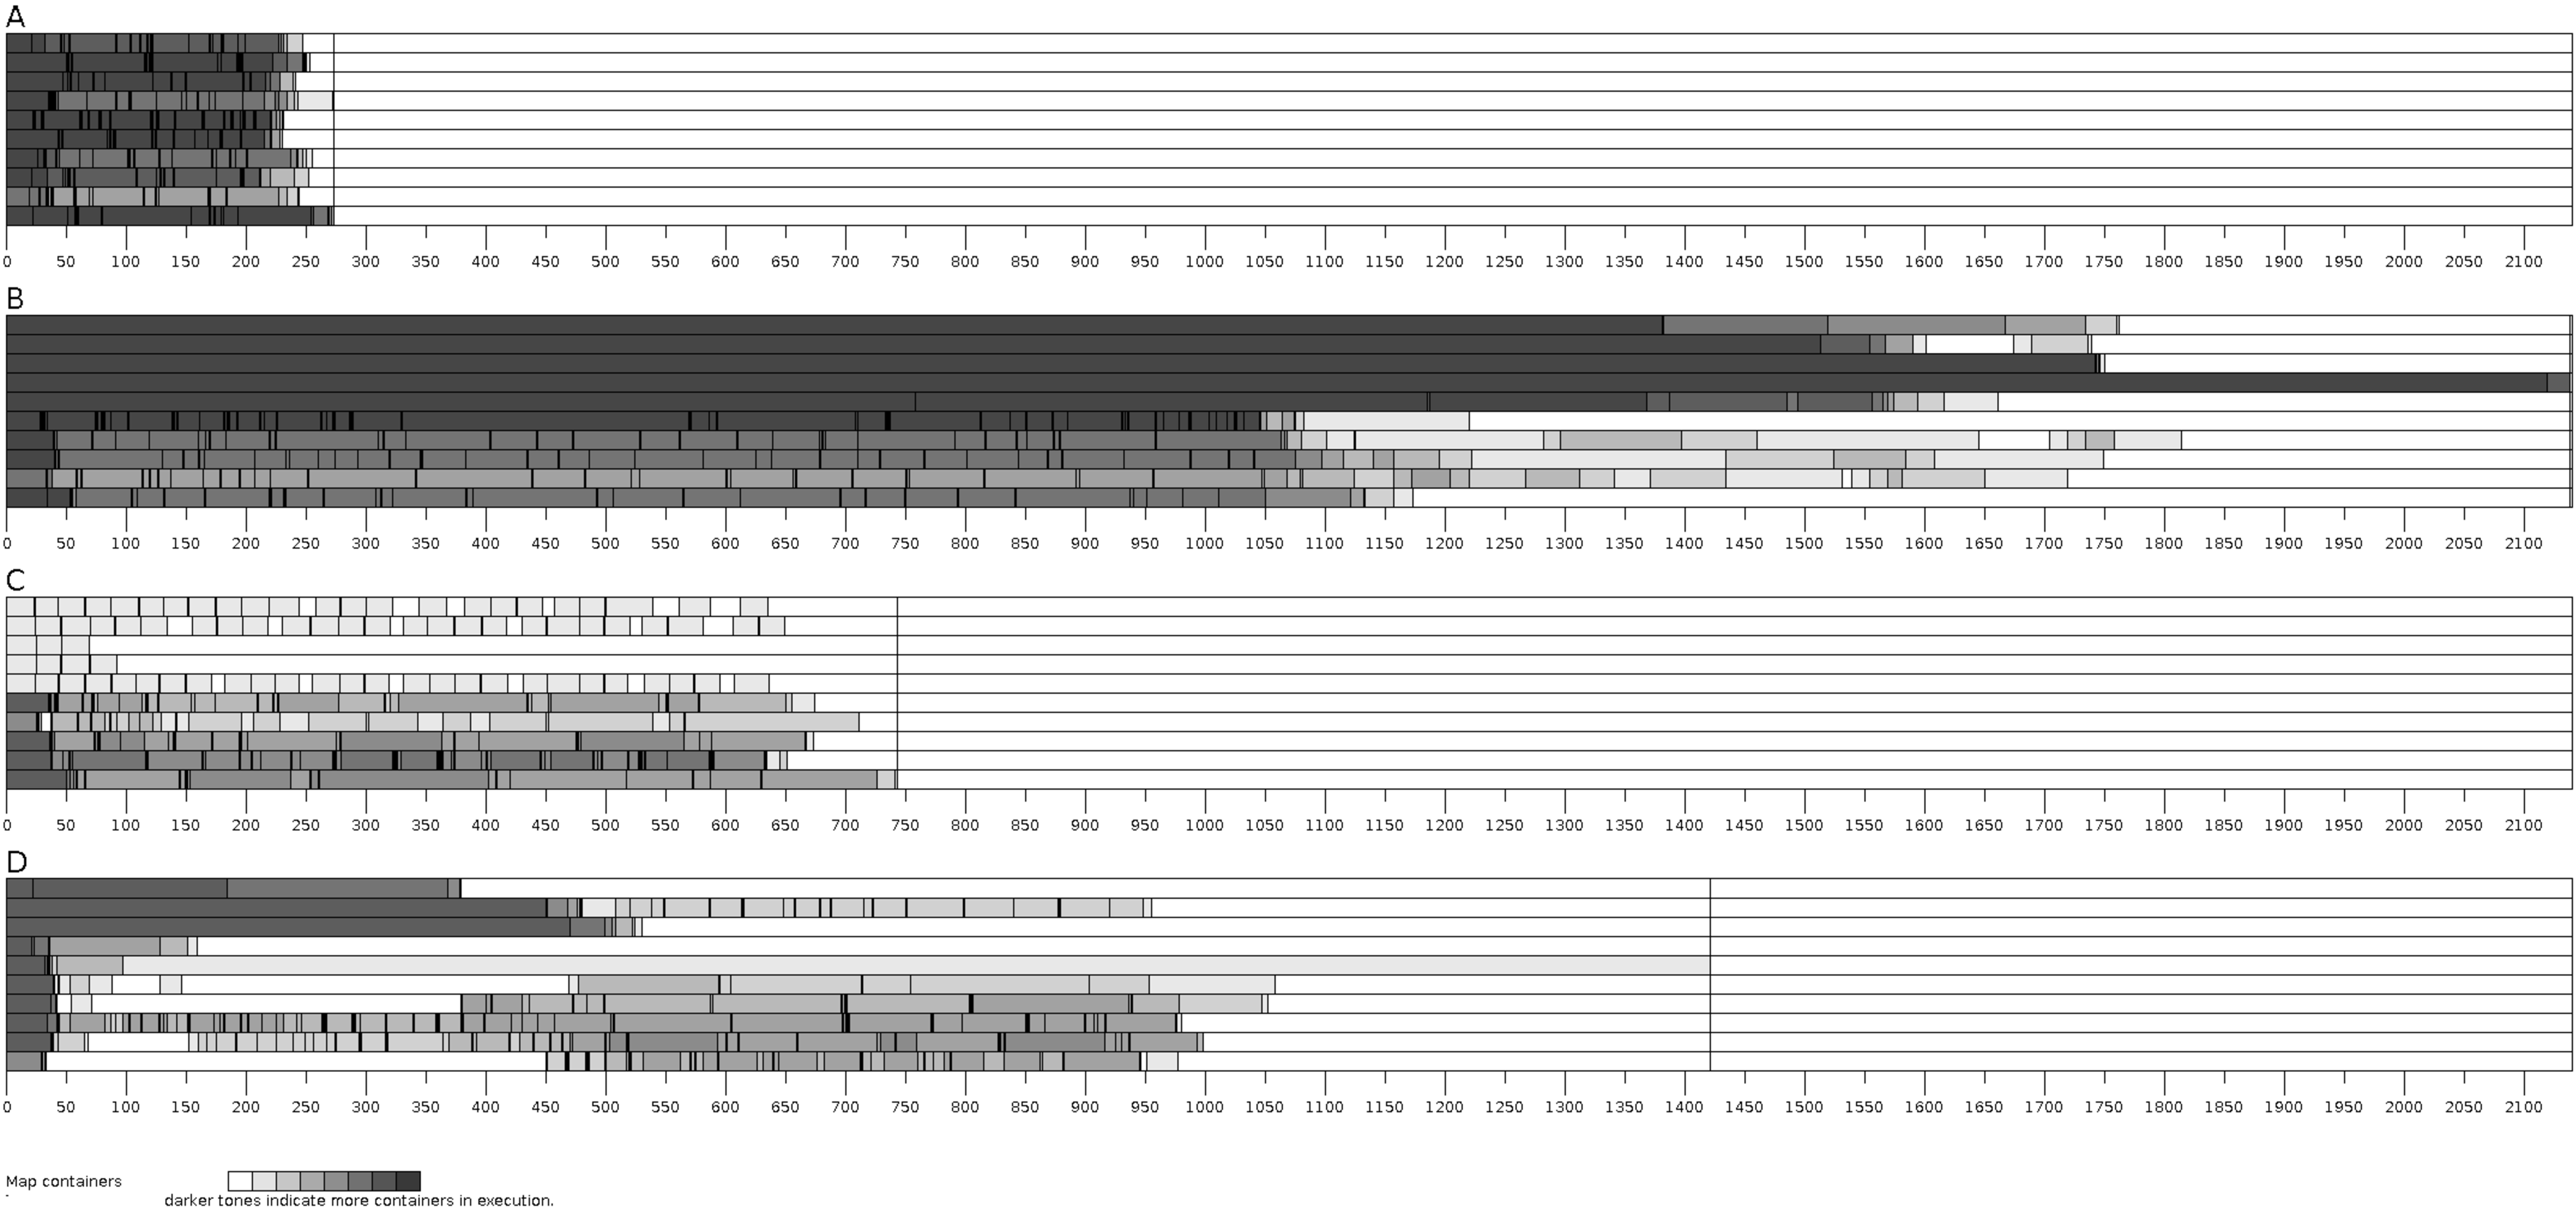
\includegraphics[width=1\textheight]{img/TS-esc-amb-full.pdf}
	\caption{Gantt charts for TeraSort on the shared environment experiment}
	\label{fig:exp2}
\end{sidewaysfigure}
\clearpage


Both Figure \ref{fig:exp2} and Table \ref{tab:exp2} show that the general behavior observed in the previous experiment is maintained. Scenario A has the fastest execution time, followed by Scenarios C, D then B. Scenarios A and C have similar averages on Map Time, followed by Scenarios D then B. 

One may wonder why a small number of containers being executed on the first 5 nodes from Scenario C while the second half has a higher load. Actually, the nodes have all resources fully used but the Gantt only shows the Map tasks to simplify the view. If we included the Reduce tasks, the average load would be the same on all these nodes. 

Nevertheless, we can observe some anomalies on Scenario D. While it was expected that the containers take a longer time to complete on the shared nodes, sometimes the second half of nodes (the dedicated ones) presented an abnormal small load in some nodes, sometimes even with zero running containers. 
This behavior can be explained by the way the Capacity Scheduler handles resource information. As explained in Section \ref{sec:desenv}, our context-awareness collector updates the resource capabilities from each node to the Capacity Scheduler. More specifically, this information is stored in a global \textit{totalResources} variable that is used by the Capacity Scheduler along with a second \textit{usedResources} variable. If an update reduces the amount of global available resources, there is a transition period in which \textit{usedResources} has a higher value than \textit{totalResources}, leading to a halt on containers deployment as the scheduler believes that there are no free resources to command. Eventually the running containers finish their work and the Capacity Scheduler will be able to start new tasks, normalizing the situation.

There are several strategies to to minimize such anomaly. The simpler strategy considers that the update algorithm gradually reduces the available resources in order to prevent a halt on the containers scheduling. Indeed, the reduction pace according to the average execution time of containers, instead of drastically modifying the available resources. The best solution, however, requires a change on the Capacity Scheduler algorithm to allow distinct lists of \textit{usedResources} and \textit{totalResources} by node. Using these detailed lists, the scheduler knowns when to stop launching a container in an overloaded node while keeping the deployment on other nodes.

\subsection{Discussions} \label{sec:disc}
Results presented in Section \ref{sec:exper} demonstrate that, by observing context information during application execution, it is possible to improve job scheduling on Hadoop framework. Indeed, the experiments prove that by tracking the changes in the available resources (core CPUs and memory), we could keep Hadoop scheduler aware of the current status of these resources. Hadoop scheduler could then base its decisions on more accurate information, corresponding to the real execution context and not to a standard one extracted from configuration files. This allowed us to obtain important performance gains, about 40\% in the TeraSort experiment, for instance. This ability to observe context information is particularly important when executing on heterogeneous or non-dedicated clusters, in which resources may fluctuate during the application execution. Offering accurate information about the environment allows Hadoop scheduler to adapt itself to the current environment even if the execution conditions change after the job starts. 

These results, although positive, have been based on a limited set of context information, the number of available cores and memory. These criteria correspond to those traditionally used by  scheduling, and in this work we focus on changing only the parameter feeding of the scheduler, keeping unchanged the scheduling policy itself. This process allows the assessment of the impact of real-time context information on the performance. Even though, other context information can be acquired thanks to our context collector and could be used for scheduling purposes. For instance, information such as network bandwidth or latency, available storage and average CPU load could be used. 

For instance, researches on Cloud Computing (\cite{Maurer2012, Assuncao2012}) propose different scheduling policies to optimize resources use and to respect signed SLA (Service Level Agreement). \cite{Maurer2012} underlines the potential effects of external factors such as workload and environmental changes on VM allocation and performance. These authors \cite{Maurer2012} consider workload volatility on resource allocation and reconfiguration in order to avoid under- or over-utilization of resources. In addition to workload information, which can be estimated using average CPU load and memory consumption, other context information can be considered. \cite{Assuncao2012} mention, for instance, the time of the day, other executing applications or the user's location. These authors suggest using context information for an adaptive job scheduling in order to rationalize resource consumption in the cloud. They assume that context-aware job scheduling is necessary in pervasive environments, in which limited mobile-based devices may delegate processing components to a cloud infrastructure. In this case, an adaptive job scheduling can be used to rationalize the consumption of cloud resources (and to avoid job violation events) based on the possible variations of the end user's local context. 
 
These works (\cite{Maurer2012, Assuncao2012, Cavallo2015}) illustrate the possible use of different context information on job scheduling. However, they also underline the necessity of an appropriate scheduling policy, specifically designed in order to explore context information. In the case of a MapReduce application in heterogeneous environments, several context parameters can be considered as relevant, and notably network conditions and data locality in addition to CPU and memory related information (e.g. available cores, CPU load, available memory, etc.). The challenge here is to figure out an adaptive scheduling policy capable of exploring this context information in an appropriate and advantageous way.  

Finally, our results (cf. Section \ref{sec:exper}) demonstrate that it is possible to adapt Hadoop scheduler for efficient execution on heterogeneous environments. The possibility of executing MapReduce applications in such environments underlines the potential of using pervasive grids for MapReduce, and more generally, for Big Data. 

Indeed, MapReduce applications, and particularly those based on the Hadoop framework, have been heavily used for Big Data to analyze large volumes of data, often unstructured, obtained from various heterogeneous sources (IoT devices, social media, etc.). These applications are mostly executed on homogeneous computing environments such as cloud computing platforms. Different reasons motivate the use of cloud computing for MapReduce applications, among them the elasticity and the cost-effectiveness. Indeed, thanks to cloud computing platforms such as Amazon Elastic MapReduce\footnote{http://aws.amazon.com/elasticmapreduce/}, it is possible to analyze an increasing volume of data, without the need of a local (and costly) infrastructure like a dedicated cluster that remains often underutilized in many organizations. Nevertheless, as underlined by \cite{Hofmann2010}, cloud computing also has several trade offs, including security, performance instability and and limited latency/throughput network performances.  \cite{Hofmann2010}, \cite{Schadt2010} also underline security and privacy issues of cloud platforms. As the indicate, several cloud providers find it hard to meet standards for auditability or to comply with legislation in the domain of security and privacy, raising the question of data sensibility. 

In other words, although interesting, homogeneous cloud platform are not the only possible solution for data analysis. Several other solutions exist, such as using off the shelf GPU-based architectures (\cite{Engel2015}) or pervasive grids (\cite{Steffenel20151034}). In this paper, we demonstrate that, with an appropriate scheduling mechanism, pervasive grids can be used for Hadoop  applications. Indeed, by introducing context-awareness capabilities, pervasive grids may represent a complementary alternative to costly dedicated clusters or to cloud infrastructures, particularly when these cannot be used due to data constraints. 


\subsection{Conclusion} \label{sec:concl}
In this work, we aimed at developing the ability to detect and adapt to resource availability changes on the environment of Apache Hadoop Capacity Scheduler. The improvements were implemented with a light-weight context collector and communication provided by ZooKeeper. These improvements go further than our previous work \cite{UBICOMM2014} by including a continuous observation of node capabilities.  
The results show that this solution can positively impact the execution performance of MapReduce applications, especially in situations where the available resources drop after the beginning of the execution. 

While Hadoop does not perform preemption/migration of tasks, the association of a context-aware scheduler and speculative tasks may contribute to circumvent the bottlenecks caused by the resources variability. Our future works will concentrate on modifying the scheduler algorithms, in order to consider a wider collection of context information than the current memory and cores parameters. We believe that additional parameters such as CPU speed, network speed and even battery capacity are essential factors in a pervasive grid. Finally, we intend to evaluate our context-aware scheduler under realistic situations with both MapReduce applications and pervasive grid environments composed of heterogeneous off-the-shelf volunteer computers.   





